\section{Companies Reference}

Selecting "Companies" from the navigation drawer opens the Companies management view. This page serves as a central reference table for railroad equipment manufacturers, locomotive builders, and operating railway companies. It displays the company short Name (abbreviation), Full Name, Type classification (e.g., Builder, Railway), Location, and Action controls. Figure \ref{fig:companies} illustrates the main Companies page interface.

\begin{figure}[H]
    \centering
    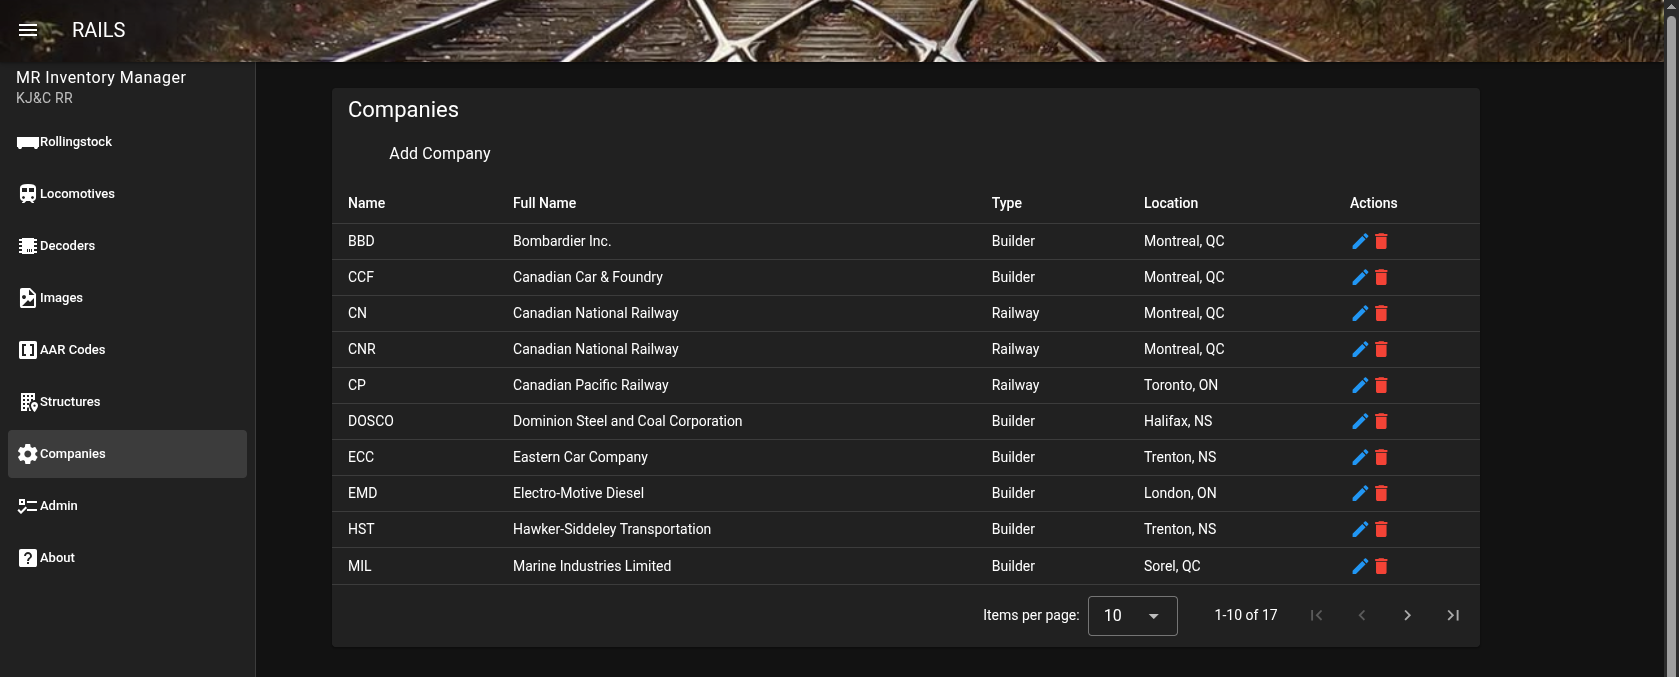
\includegraphics[width=0.85\textwidth]{./images/companies.png}
    \caption{Companies Page}
    \label{fig:companies}
\end{figure}

\subsection{Adding a Company}

Clicking the "Add Company" button above the table opens a modal dialog to define a new corporate entry. The form prompts for the company's short Name, Long Name, Type (such as Builder or Railway), and headquarters Location. Figure \ref{fig:companies-new} shows the company entry modal.

\begin{figure}[H]
    \centering
    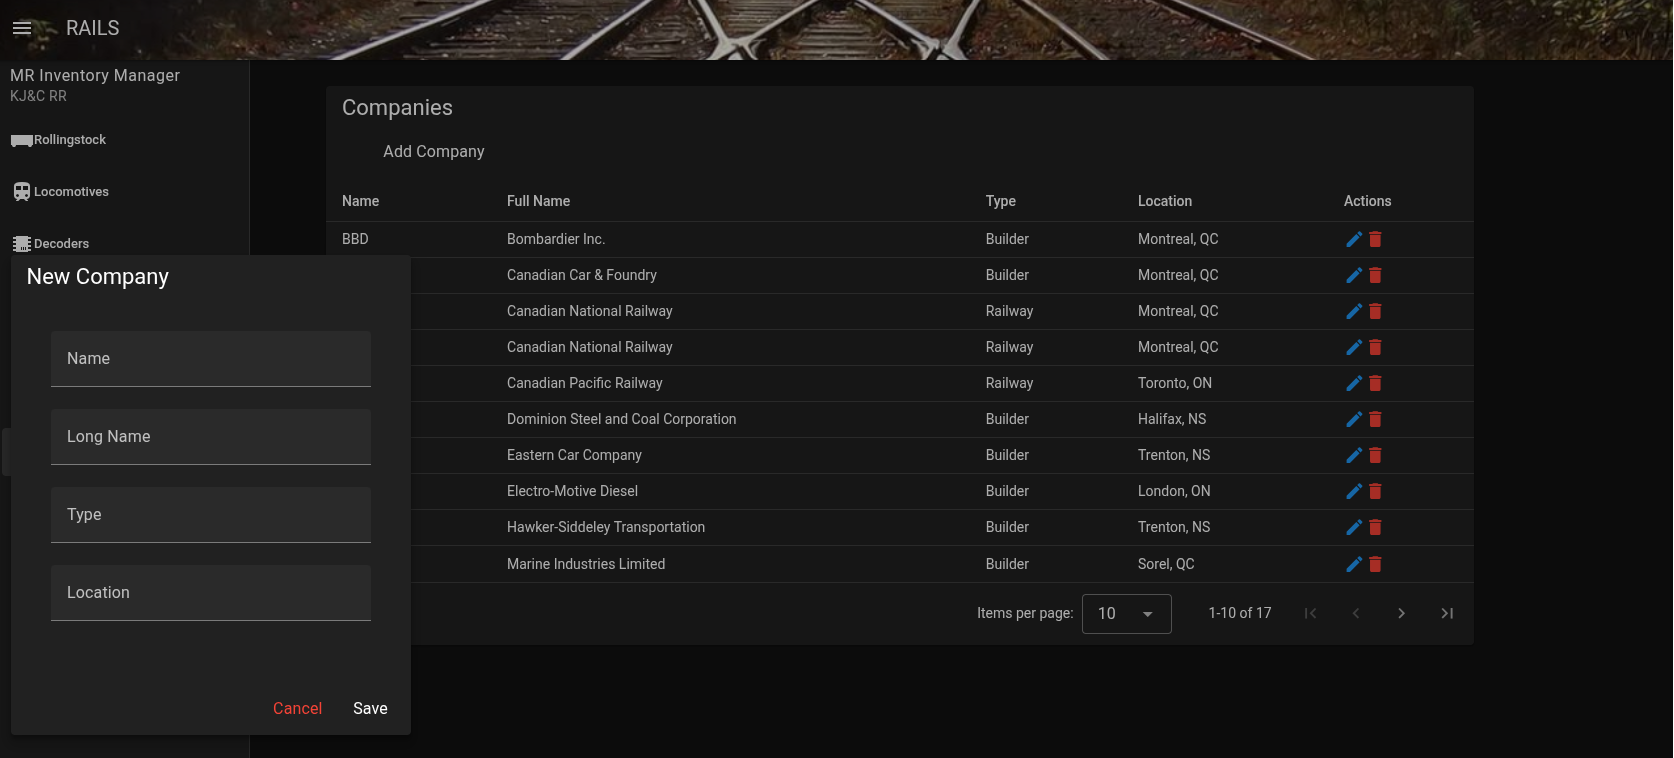
\includegraphics[width=0.85\textwidth]{./images/companies-new.png}
    \caption{Add Company Dialog}
    \label{fig:companies-new}
\end{figure}

\subsection{Editing Company Records}

To modify an existing company entry, click the blue pencil icon under the Actions column. This opens the edit dialog populated with current information, allowing adjustments to reporting marks, full corporate titles, or location details. Figure \ref{fig:companies-edit} displays the edit company interface.

\begin{figure}[H]
    \centering
    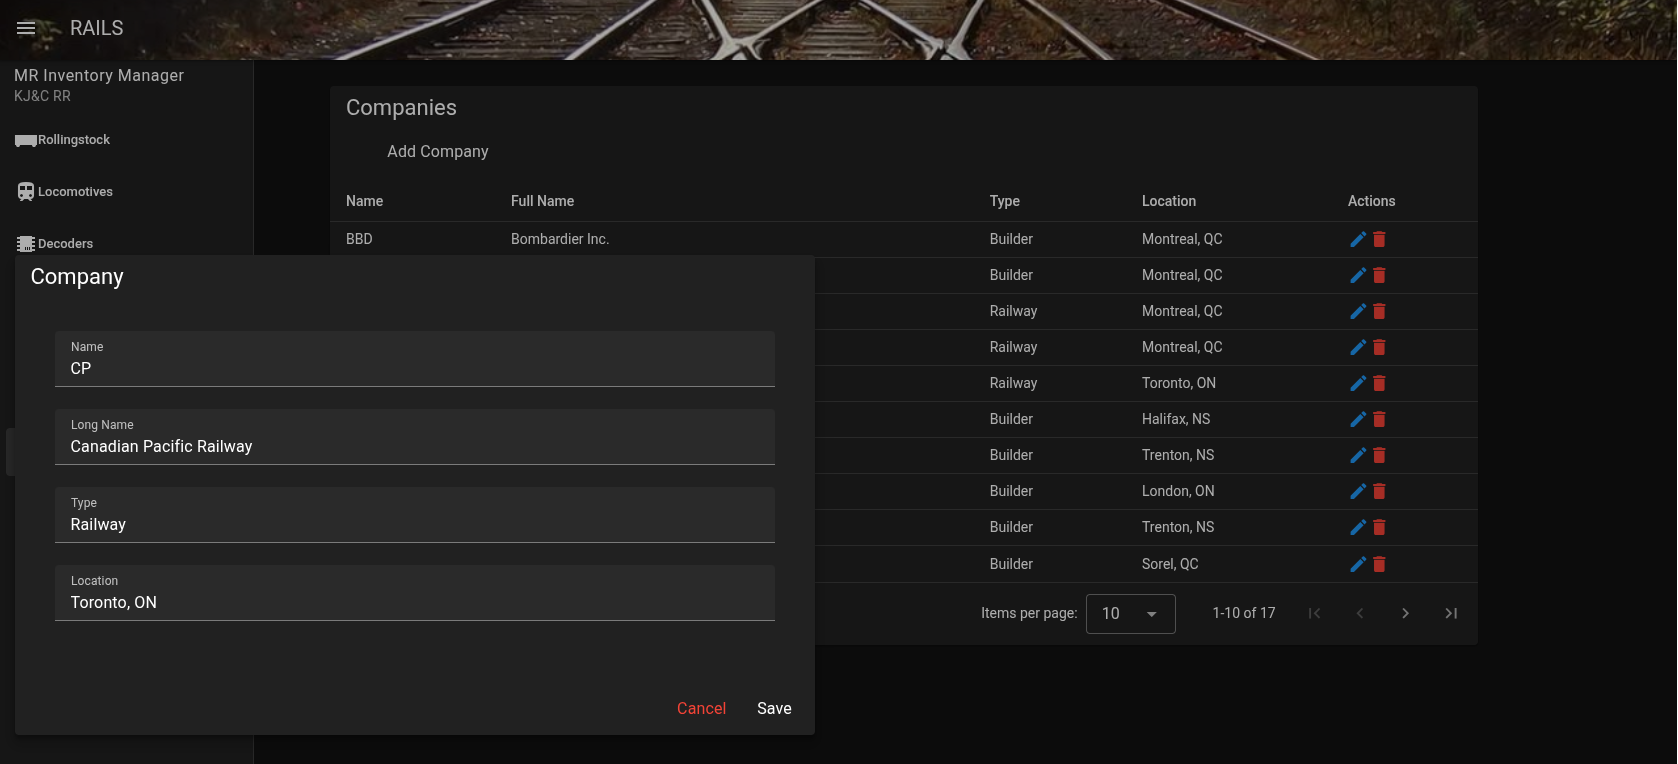
\includegraphics[width=0.85\textwidth]{./images/companies-edit.png}
    \caption{Edit Company}
    \label{fig:companies-edit}
\end{figure}

\subsection{Deleting Company Records}

To remove a corporate entity from the system reference table, click the red trash bin icon in the Actions column. A confirmation prompt appears asking for verification before removing the company entry. Figure \ref{fig:companies-delete} shows the deletion confirmation prompt dialog.

\begin{figure}[H]
    \centering
    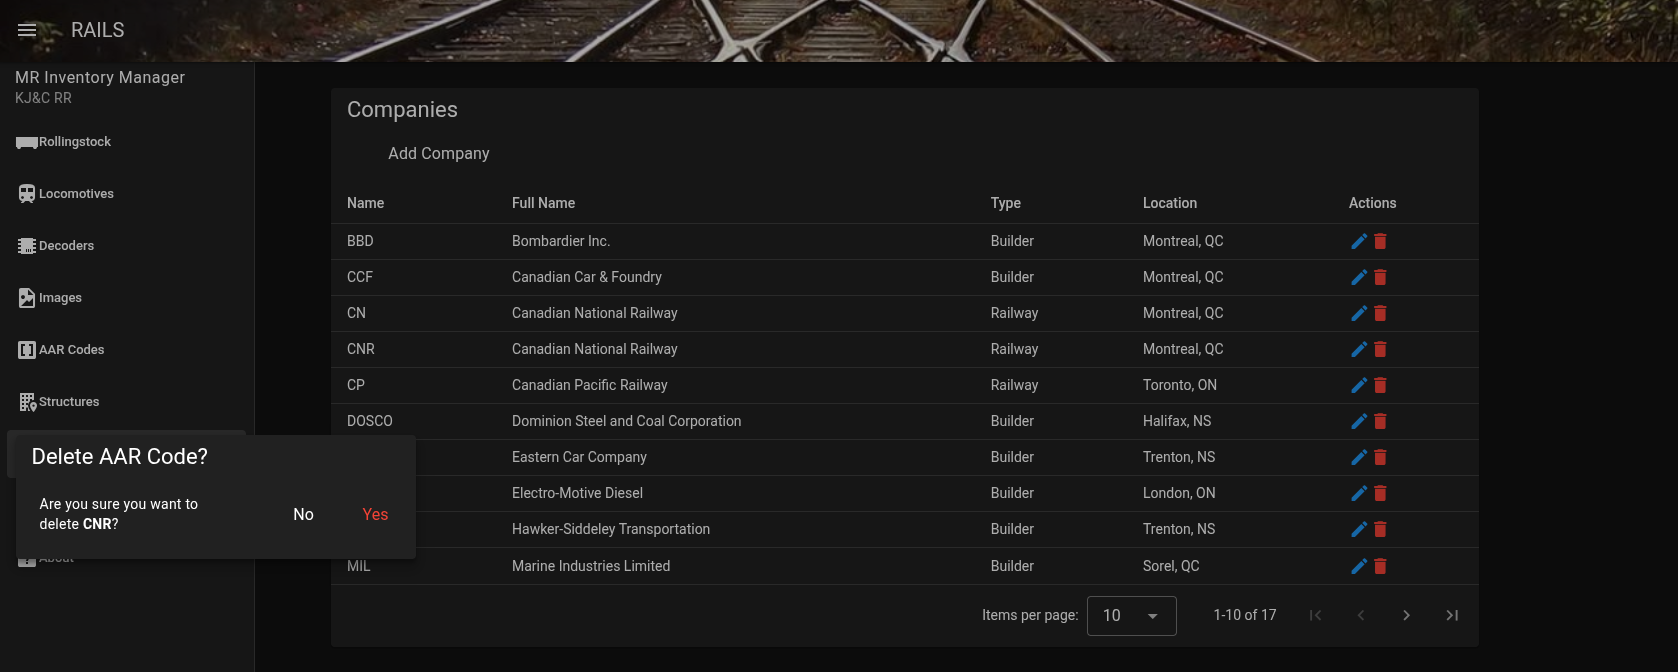
\includegraphics[width=0.85\textwidth]{./images/companies-delete.png}
    \caption{Delete Company Confirmation}
    \label{fig:companies-delete}
\end{figure}
